\documentclass[dutch]{beamer}
\usepackage{babel}
\usepackage{graphicx}
\usepackage{epsfig}

\usetheme{Rochester}
\useinnertheme{rounded}
\usefonttheme{structurebold}
\usecolortheme{beetle}

\newtheorem{stelling}[theorem]{Stelling}

\theoremstyle{definition}
\newtheorem{definitie}[theorem]{Definitie}

\theoremstyle{remark}
\newtheorem{opmerking}[theorem]{Opmerking}

\theoremstyle{example}
\newtheorem{voorbeeld}[theorem]{Voorbeeld}


\AtBeginSection[]{\plainframe{\tableofcontents[currentsection,hidesubsections]}}

\title{Similariteitsgebaseerd rangschikken van beelden in zoekmachines}
\author{Klaas Bosteels}
\date{Academiejaar 2005-2006}

\titlegraphic{\includegraphics[scale=1]{ugent.eps}}

\begin{document}

\plainframe{\titlepage}

\section{Inleiding}
\frame
{
  \frametitle{Situering}
  
  \begin{center}
  \includegraphics[width=\textwidth]{images/situering.eps}
  \end{center}
}
\subsection{Tekstgebaseerd zoeken van beelden}
\frame
{
  \frametitle{Tekstgebaseerd zoeken van beelden}

  \begin{center}
  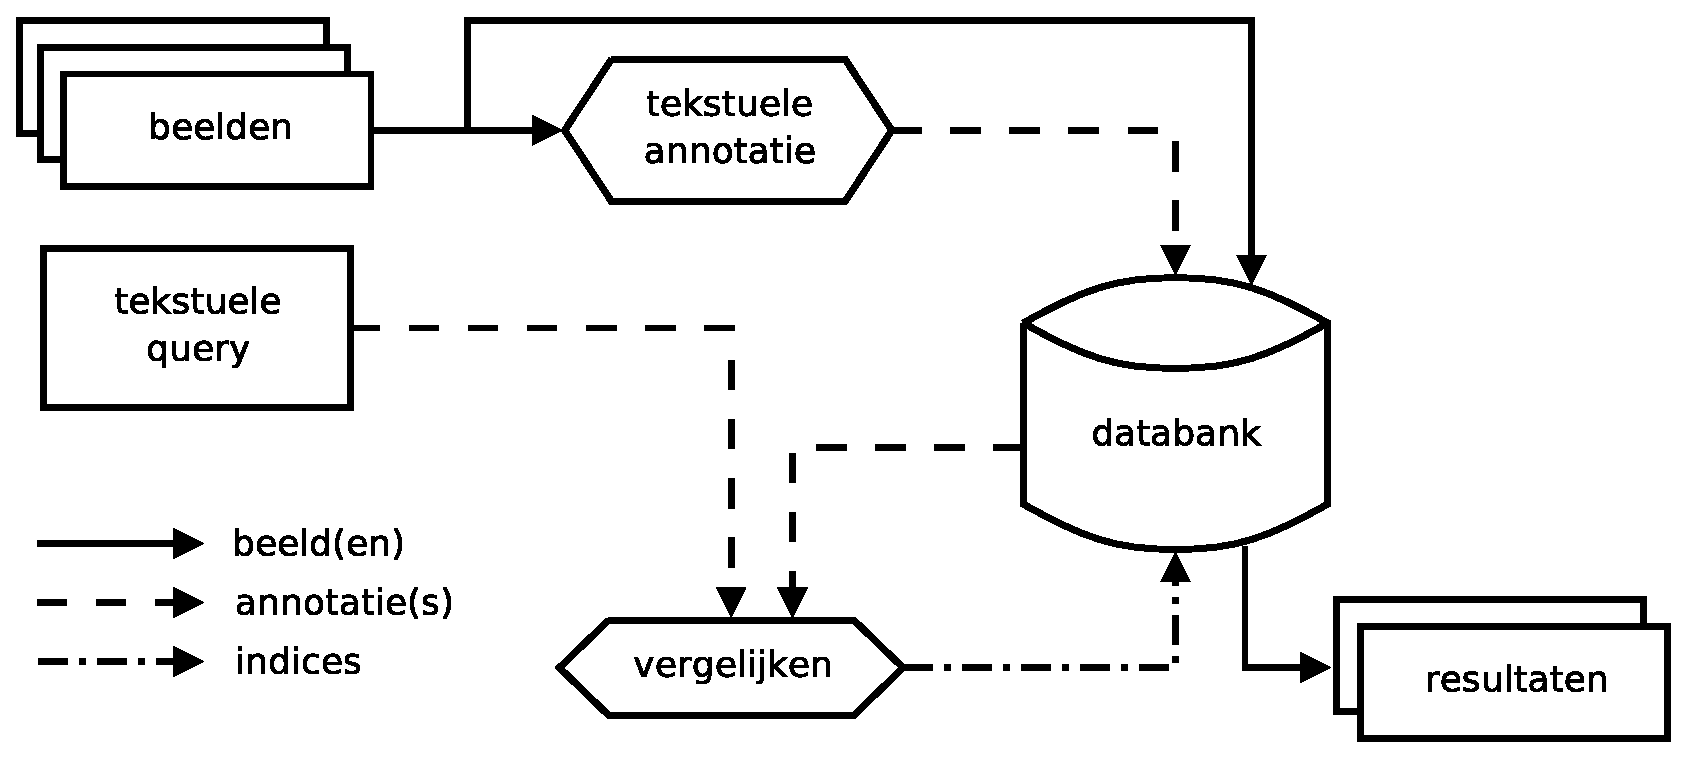
\includegraphics[width=\textwidth]{images/tbir.eps}
  \end{center}

  Terminologie: Text-Based Image Retrieval (TBIR).
}
\subsection{Inhoudgebaseerd zoeken van beelden}
\frame
{
  \frametitle{Inhoudgebaseerd zoeken van beelden}

  \begin{center}
  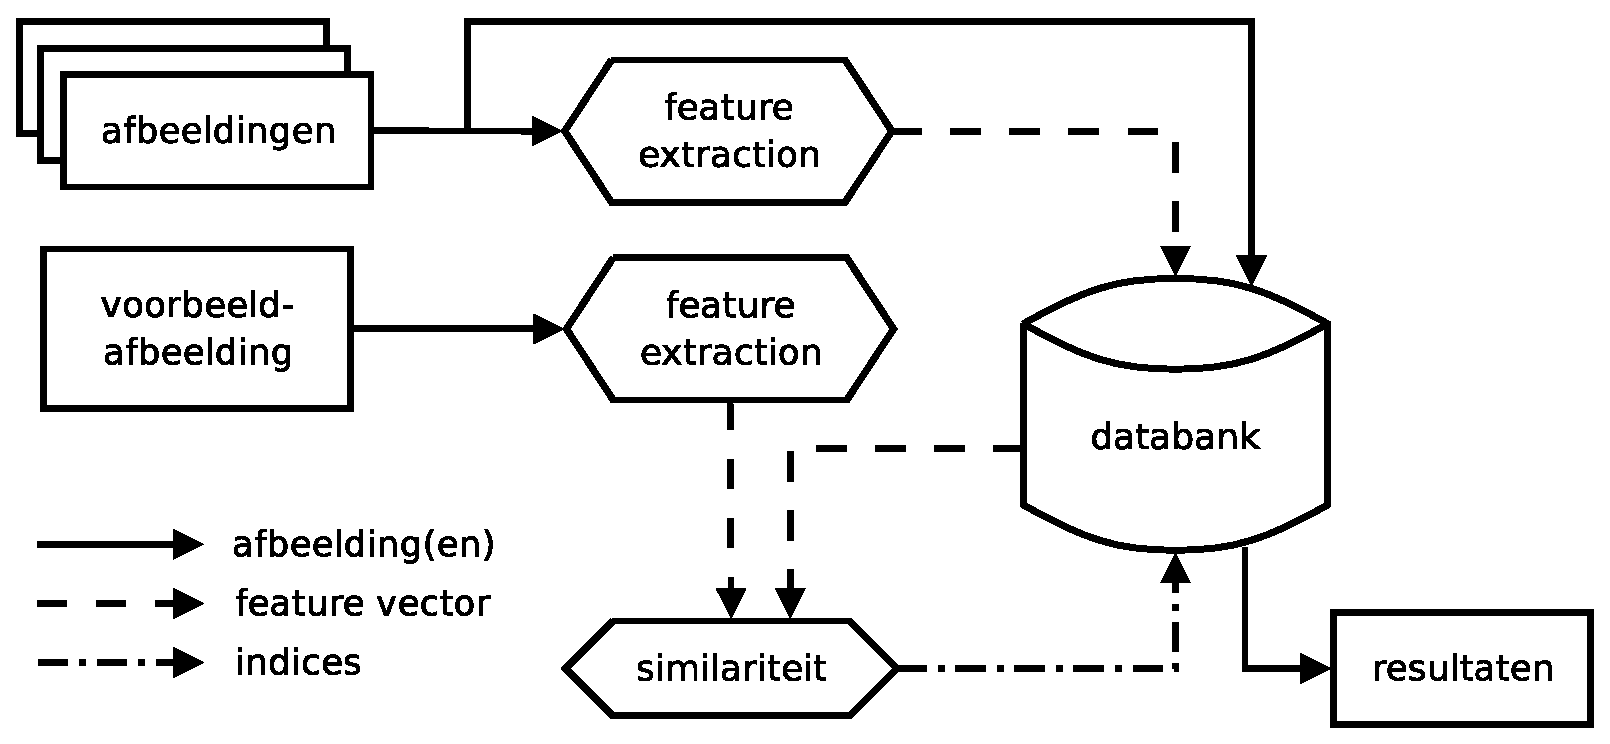
\includegraphics[width=\textwidth]{images/cbir.eps}
  \end{center}

  Terminologie: Content-Based Image Retrieval (CBIR).
}
\subsection{Similariteitsgebaseerd rangschikken van de zoekresultaten}
\frame
{
  \frametitle{Similariteitsgebaseerd rangschikken van de zoekresultaten}
}

\section{Wiskundige fundamenten}
\frame
{
  \frametitle{Wiskundige fundamenten}

  Basisidee:
  \begin{enumerate}
  \item Beelden identificeren met \textbf{(L-)vaagverzamelingen}.
  \item Gebruik maken van \textbf{vaagsimilariteitsmaten} om de graduele 
  gelijkenis tussen die vaagverzamelingen te bepalen.
  \end{enumerate}
  
  \textbf{Aggregatieoperatoren} laten toe om
  \begin{itemize}
  \item verschillende similariteitsmaten te combineren
  \item en meerdere voorbeelden te ondersteunen.
  \end{itemize}
  
  \begin{opmerking}
  Notaties: $A^c = co_{N_s} A$, $A \cap B = A \cap_{T_M} B$, $A \cup B = A \cup_{S_M} B$,
  $A \setminus B = A \cap B^c$ en $A \triangle B = (A \setminus B) \cup (B \setminus A)$,
  met $A$ en $B$ vaagverzamelingen in een zelfde universum, $N_s$ de standaardnegator, 
  $T_M$ het minimum en $S_M$ het maximum.
  \end{opmerking}
}

\section{Enkele begrippen uit beeldverwerking}
\subsection{Modellering van kleuren en beelden}
\subsection{Kleurkwantisatie}
\subsection{Lineaire filters}
\subsection{Randdetectie}

\section{Similariteitsmaten voor beelden}
\subsection{Definitie en eigenschappen}
\frame
{
  \frametitle{Definitie en eigenschappen}

  \begin{definitie}
  Een \textbf{similariteitsmaat voor beelden} is een maat die de gelijkenis 
  tussen twee gegeven beelden uitdrukt als een getal in het eenheidsinterval 
  $[0,1]$.
  \end{definitie}

  Eigenschappen:
  \begin{itemize}
  \item Reflexief: $M(A,A)=1$
  \item Symmetrisch: $M(A,B)=M(B,A)$
  \item Niet (noodzakelijk) transitief!
  \end{itemize}
  
  \begin{opmerking}
  In het vervolg bedoelen we met ``similariteitsmaat'' steeds een similariteitsmaat
  voor beelden (en niet een vaagsimilariteitsmaat).
  \end{opmerking}
}
\subsection{Evaluatie van performantie}
\frame
{
  \frametitle{Evaluatie van performantie: testcollectie}

  Testcollectie van $N$ beelden die corresponderen met 
  $N/N_R$ objecten die elk $N_R$ keer gefotografeerd werden:

\begin{center}

\begin{tabular}{c@{\ }c@{}c@{}c@{}c@{}c c@{\ }c@{}c@{}c@{}c@{}c}

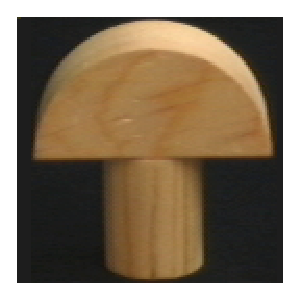
\includegraphics[width=0.8cm]{coil/beeld-0.eps} &
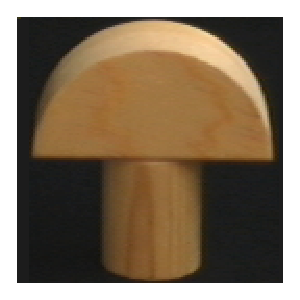
\includegraphics[width=0.8cm]{coil/beeld-1.eps} &

\includegraphics[width=0.8cm]{coil/beeld-2.eps} &
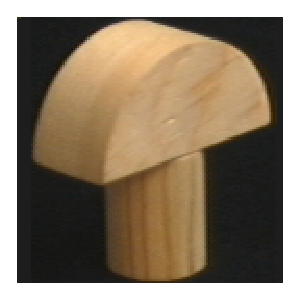
\includegraphics[width=0.8cm]{coil/beeld-3.eps} &
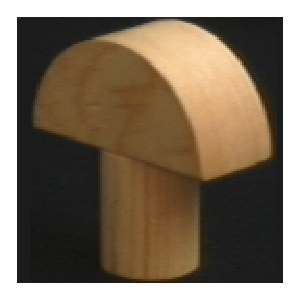
\includegraphics[width=0.8cm]{coil/beeld-4.eps} &

\includegraphics[width=0.8cm]{coil/beeld-5.eps} &

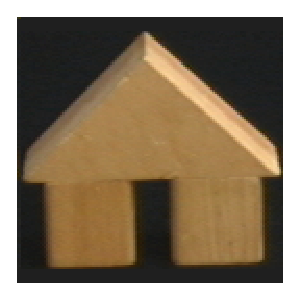
\includegraphics[width=0.8cm]{coil/beeld-42.eps} &
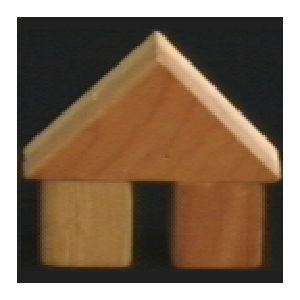
\includegraphics[width=0.8cm]{coil/beeld-43.eps} &

\includegraphics[width=0.8cm]{coil/beeld-44.eps} &
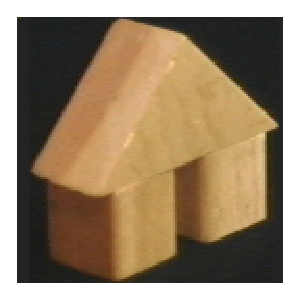
\includegraphics[width=0.8cm]{coil/beeld-45.eps} &
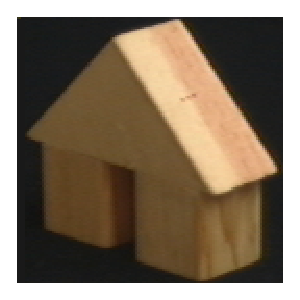
\includegraphics[width=0.8cm]{coil/beeld-46.eps} &
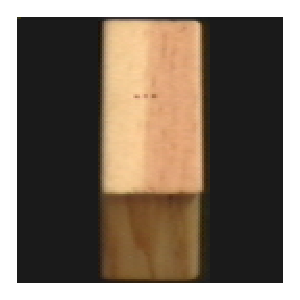
\includegraphics[width=0.8cm]{coil/beeld-47.eps} \\

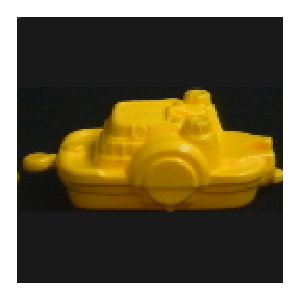
\includegraphics[width=0.8cm]{coil/beeld-12.eps} &
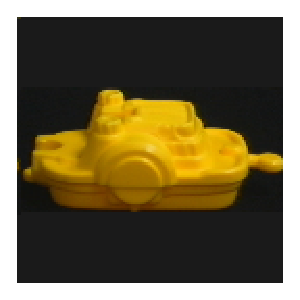
\includegraphics[width=0.8cm]{coil/beeld-13.eps} &
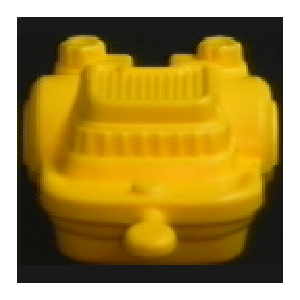
\includegraphics[width=0.8cm]{coil/beeld-14.eps} &
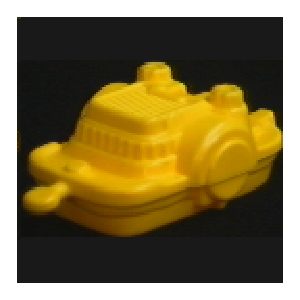
\includegraphics[width=0.8cm]{coil/beeld-15.eps} &
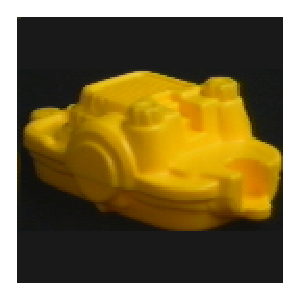
\includegraphics[width=0.8cm]{coil/beeld-16.eps} &
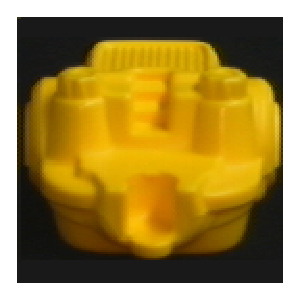
\includegraphics[width=0.8cm]{coil/beeld-17.eps} &


\includegraphics[width=0.8cm]{coil/beeld-18.eps} &

\includegraphics[width=0.8cm]{coil/beeld-19.eps} &
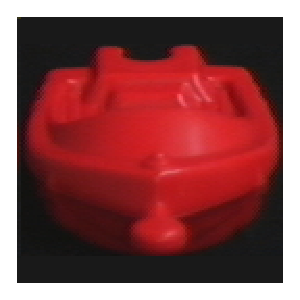
\includegraphics[width=0.8cm]{coil/beeld-20.eps} &
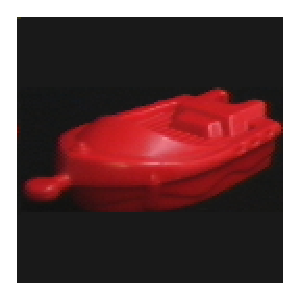
\includegraphics[width=0.8cm]{coil/beeld-21.eps} &
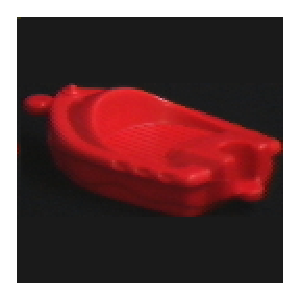
\includegraphics[width=0.8cm]{coil/beeld-22.eps} &
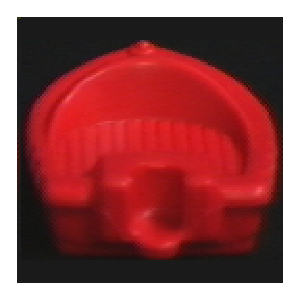
\includegraphics[width=0.8cm]{coil/beeld-23.eps} \\

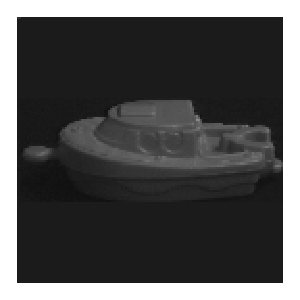
\includegraphics[width=0.8cm]{coil/beeld-24.eps} &
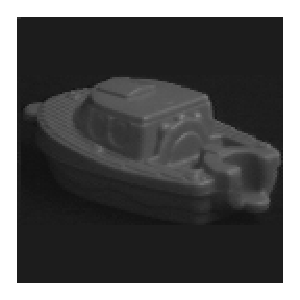
\includegraphics[width=0.8cm]{coil/beeld-25.eps} &
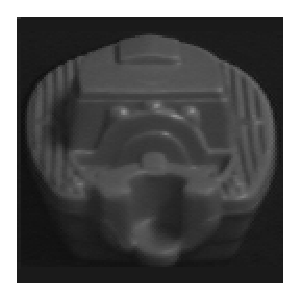
\includegraphics[width=0.8cm]{coil/beeld-26.eps} &
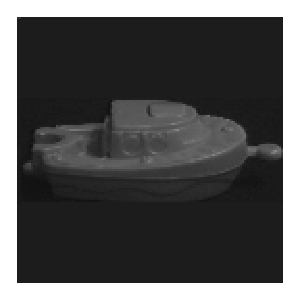
\includegraphics[width=0.8cm]{coil/beeld-27.eps} &
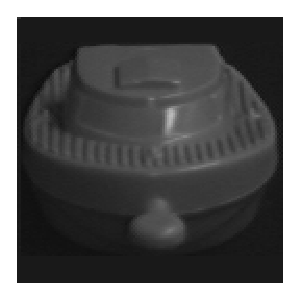
\includegraphics[width=0.8cm]{coil/beeld-28.eps} &
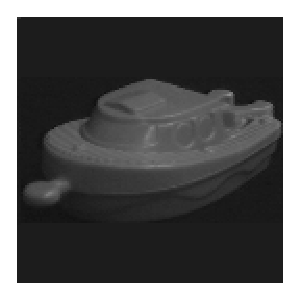
\includegraphics[width=0.8cm]{coil/beeld-29.eps} &

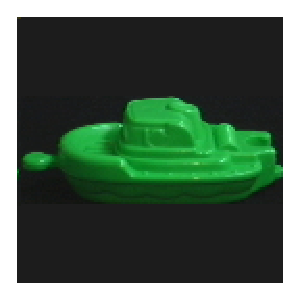
\includegraphics[width=0.8cm]{coil/beeld-54.eps} &
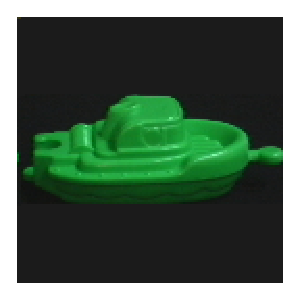
\includegraphics[width=0.8cm]{coil/beeld-55.eps} &
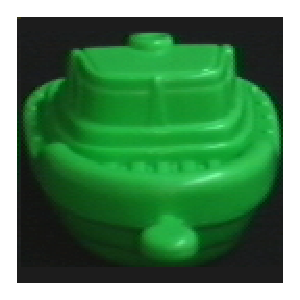
\includegraphics[width=0.8cm]{coil/beeld-56.eps} &
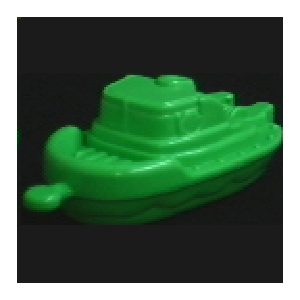
\includegraphics[width=0.8cm]{coil/beeld-57.eps} &
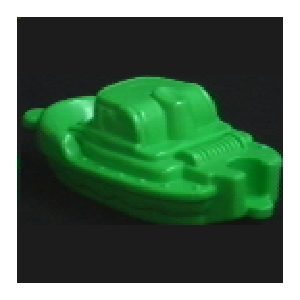
\includegraphics[width=0.8cm]{coil/beeld-58.eps} &
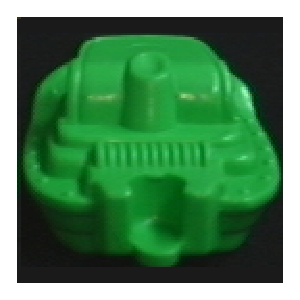
\includegraphics[width=0.8cm]{coil/beeld-59.eps} \\

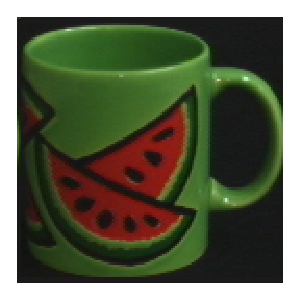
\includegraphics[width=0.8cm]{coil/beeld-30.eps} &
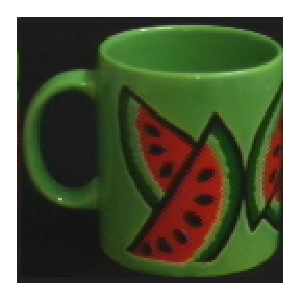
\includegraphics[width=0.8cm]{coil/beeld-31.eps} &
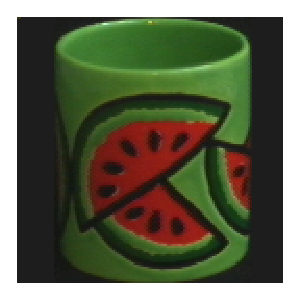
\includegraphics[width=0.8cm]{coil/beeld-32.eps} &
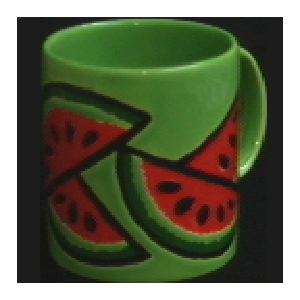
\includegraphics[width=0.8cm]{coil/beeld-33.eps} &
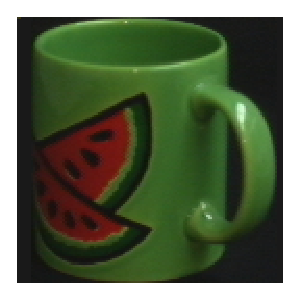
\includegraphics[width=0.8cm]{coil/beeld-34.eps} &
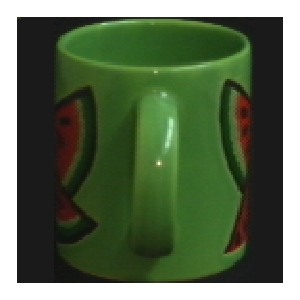
\includegraphics[width=0.8cm]{coil/beeld-35.eps} &

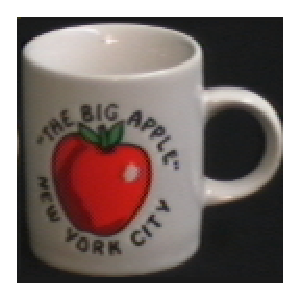
\includegraphics[width=0.8cm]{coil/beeld-36.eps} &
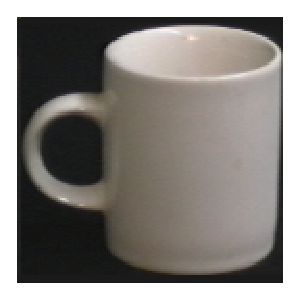
\includegraphics[width=0.8cm]{coil/beeld-37.eps} &
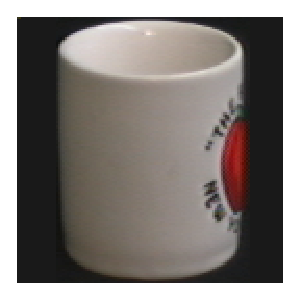
\includegraphics[width=0.8cm]{coil/beeld-38.eps} &
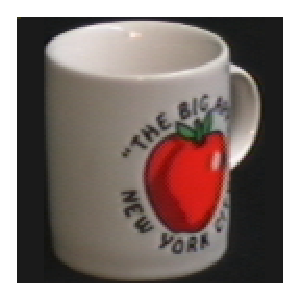
\includegraphics[width=0.8cm]{coil/beeld-39.eps} &
\includegraphics[width=0.8cm]{coil/beeld-40.eps} &
\includegraphics[width=0.8cm]{coil/beeld-41.eps} \\

\includegraphics[width=0.8cm]{coil/beeld-6.eps} &
\includegraphics[width=0.8cm]{coil/beeld-7.eps} &
\includegraphics[width=0.8cm]{coil/beeld-8.eps} &
\includegraphics[width=0.8cm]{coil/beeld-9.eps} &
\includegraphics[width=0.8cm]{coil/beeld-10.eps} &
\includegraphics[width=0.8cm]{coil/beeld-11.eps} &

\includegraphics[width=0.8cm]{coil/beeld-48.eps} &
\includegraphics[width=0.8cm]{coil/beeld-49.eps} &
\includegraphics[width=0.8cm]{coil/beeld-50.eps} &
\includegraphics[width=0.8cm]{coil/beeld-51.eps} &
\includegraphics[width=0.8cm]{coil/beeld-52.eps} &
\includegraphics[width=0.8cm]{coil/beeld-53.eps} \\

\includegraphics[width=0.8cm]{coil/beeld-60.eps} &
\includegraphics[width=0.8cm]{coil/beeld-61.eps} &
\includegraphics[width=0.8cm]{coil/beeld-62.eps} &
\includegraphics[width=0.8cm]{coil/beeld-63.eps} &
\includegraphics[width=0.8cm]{coil/beeld-64.eps} &
\includegraphics[width=0.8cm]{coil/beeld-65.eps} &
\multicolumn{2}{c}{$N_R = 6$} & 
\multicolumn{4}{c}{$N = 11 \cdot N_R = 66$}

\end{tabular}
\end{center}

}
\frame
{
  \frametitle{Evaluatie van performantie: GGR}

  We gebruiken een similariteitsmaat om de testcollectie te rangschikken volgens
  similariteit met een voorbeeld. Beschouw nu de vector 
  $(r_1,r_2,\ldots,r_{N_R}) \in \{1,2,\ldots,N\}^{N_R}$, 
  waarbij $r_i$ het rangnummer van het $i$-de relevante beeld voorstelt.

  \begin{definitie}
  
  De \textbf{genormaliseerde gemiddelde rang} (GGR) wordt gegeven door de volgende afbeelding:
  $$
  \small\begin{array}{lrcl}
  \textrm{GGR}: & \{1,2,\ldots,N\}^{N_R} & \to 	& [0,1] \\
		& (r_1,r_2,\ldots,r_{N_R}) & \mapsto &
	{\displaystyle\frac{1}{N \cdot N_R}\left[ \left(\sum_{i=1}^{N_R}r_i\right) - \frac{N_R \cdot (N_R + 1)}{2} \right]},\\[15pt]
	& & & \qquad \quad \forall (r_1, r_2, ..., r_{N_R}) \in \{1,2,\ldots,N\}^{N_R}
  \end{array}
  $$
  \end{definitie}
 
  De GGR nadert naar $1$ naarmate de performantie slechter wordt.
}
\frame
{
  \frametitle{Evaluatie van performantie: GGGR}

  Als het zoeken naar \includegraphics[width=0.6cm]{coil/beeld-12.eps} de volgende rangschikking geeft:
  dan

  \begin{itemize}
  \item We berekenen de GGR voor meerdere voorbeelden en beschouwen het 
  gemiddelde van de bekomen waarden. 
  \item De waarde die we zo bekomen noemen we de
  \textbf{globale genormaliseerde gemiddelde rang} (GGGR).
  \item 
  \end{itemize}
}
\subsection{Optimalisatie van performantie}
\frame
{
  \frametitle{Optimalisatie van performantie}
  
}

\section{Pixelgebaseerde similariteitsmaten}
\frame
{
  \frametitle{Pixelgebaseerde similariteitsmaten}

  Pixelgebaseerd: de pixels (spatiale lokaties) vormen het universum.

  \begin{center}
  \begin{tabular}{l@{$\qquad \qquad$}r}
  \includegraphics[height=0.3\textheight]{images/rescale.eps} & 
  \includegraphics[height=0.3\textheight]{images/dominant_colors.eps} \\
  \\
  \multicolumn{2}{c}{\includegraphics[height=0.3\textheight]{images/multires2.eps}}
  \end{tabular}
  \end{center}
}

\section{Kleurgebaseerde similariteitsmaten}
\frame
{
  \frametitle{Pixelgebaseerde similariteitsmaten}

  Kleurgebaseerd: niet de pixels maar de kleuren vormen het universum.

  \begin{center}
  \includegraphics[height=0.4\textheight]{images/histograms.eps}
  \end{center}
}

\section{Implementatie}

\end{document}
